% This work is licensed under the Creative Commons Attribution-NonCommercial 4.0 International License.
% To view a copy of this license, visit http://creativecommons.org/licenses/by-nc/4.0/
% or send a letter to Creative Commons, PO Box 1866, Mountain View, CA 94042, USA.

% !TEX TS-program = xelatex

\documentclass[../Main/chem371-notes.tex]{subfiles}

\setcounter{chapter}{1}
\begin{document}

\chapter{Solving the Schr\"{o}dinger equation for one-electron systems}

The goal of this chapter is to discuss how we can practically solve the Schr\"{o}dinger equation with a computer.
We will encounter the idea of using a basis of functions (basis set) to find approximate solutions that can be systematically improved.
Lastly, we will look at some applications of these ideas.

\section{Exact solutions to the Schr\"{o}dinger equation}
Only for a handful of models relevant to chemistry we know how to solve the Schr\"{o}dinger equation.
Some examples are a particle in a box, a particle attached to a spring (harmonic oscillator), a rotating body, any atom with one electron, and the \ce{H2+} molecule.
For example, the hydrogen atom solutions are known to depend on three quantum numbers $n$, $l$, and $m_l$, and that the energy levels (eigenvalues) are given by
\begin{iequation}
E_n = - \frac{1}{2 n^2}  \, E_\mathrm{h}, \quad n = 1, 2, \ldots
\end{iequation}
The wave function is usually expressed in \emph{spherical coordinates} ($r, \theta, \phi$)\mnote{
If you are curious, spherical coordinates are connected to Cartesian coordinates via the following equations
\begin{align*}
x & =  r \sin \theta \cos \phi, \\
y & =  r \sin \theta \sin \phi, \\
z & =  r \cos \theta
\end{align*}
\centering{
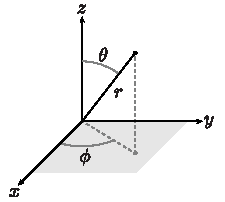
\includegraphics[width=2.0in]{img/spherical_coordinates.pdf}}
\captionof{figure}{Definition of the spherical coordinates $r$, $\theta$, and $\phi$.}
\label{fig:rigidrotor:spherical}
}
 as a product of a function that depends on the electron distance $R_{nl}(r)$ and a term that depends on the angles $Y_l^{m_l}(\theta,\phi)$
\begin{equation}
\psi_{nlm_l}(r,\theta,\phi) = R_{nl}(r) Y_l^{m_l}(\theta,\phi)
\end{equation}
For example, the wave function for the  ground state of hydrogen, the 1s orbital, is given by
\begin{equation}
\mathrm{1s} = \psi_{1,0,0}(r,\theta,\phi) = R_{1,0}(r) Y_0^0(\theta,\phi) = 2 e^{-r} \frac{1}{\sqrt{4\pi}} = \frac{1}{\sqrt{\pi}} e^{-r}
\end{equation}
while the 2p$_{z}$ orbital is given by
\begin{align}
\mathrm{2p}_{z} &= \psi_{2,1,0}(r,\theta,\phi) = R_{2,1}(r) Y_1^{0}(\theta,\phi) =
\frac{1}{4\sqrt{2 \pi}}   r e^{-r/2} \cos \theta.
\end{align}

When we turn to more complicated systems like atoms with two or more electrons and molecules the Schr\"{o}dinger equation becomes intractable and we have to turn to numerical methods to solve it.
This is what we will do in the next section.

\section{Approximate solutions via expansion in a basis}
\mfigure{
\centering{
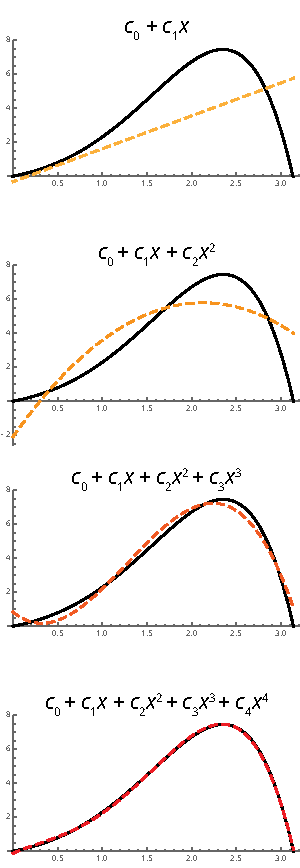
\includegraphics[width=1.75in]{img/basis_expansion.pdf}
}
\captionof{figure}{Example of expansion of the function $\exp(x) \sin(x)$ in a basis of polynomials $x^i$.
By the time we include fourth powers of $x$ this function is approximated well in the entire range $0 \leq x \leq \pi$.}
}
One way to find an approximate solution of the Schr\"{o}dinger equation is to express it as a \emph{linear combination of basis functions}.
This is a very common strategy for studying differential equations that are too difficult to solve in analytical form.
The basic idea is to approximate a function $g(x)$ as a sum of a finite number of fixed functions $f_i(x)$, called basis functions, multiplied by the coefficients $c_i$
\begin{equation}
g(x) \approx  c_1 f_1(x) +  c_2 f_2(x) + \cdots + c_K f_K(x) = \sum_{i=1}^{K} c_i f_i(x) 
\end{equation}
You can think of this approximation as fitting the function $g(x)$ with the basis functions, where the unknowns are the fitting coefficients $c_i$.
For example, we could choose the set of basis functions to be the polynomials of $x$ and stop at the polynomial of order $K$ (here we also include the constant term $x^0 = 1$)
\begin{equation}
g(x) \approx  c_0 +  c_1 x + \cdots + c_K x^{K} = \sum_{i=1}^{K} c_i x^{i-1}
\end{equation}

\section{Linear combination of atomic orbitals}

\centering{
\begin{tabular}{@{} cccc @{}} % Column formatting, @{} suppresses leading/trailing space
\toprule
Basis    & Basis Functions & Energy (\Eh) & Error (\Eh) \\
\midrule
cc-pVDZ &   5 & $-$0.499278403 & 0.000721597 \\ 
cc-pVTZ &  14 & $-$0.499809811 & 0.000190189 \\ 
cc-pVQZ &  30 & $-$0.499945569 & 0.000054431 \\ 
cc-pV5Z &  55 & $-$0.499994535 & 0.000005465 \\ 
cc-pV6Z &  91 & $-$0.499999245 & 0.000000755 \\ 
Exact &  $\infty$ & $-$0.500000000 & 0.000000000\\
\bottomrule
\end{tabular}
\captionof{table}{Convergence of the energy of the hydrogen atom as a function of the computational basis.
The exact solution corresponds to the analytic solution of the Schr\"{o}dinger equation.}
}

\centering{
\begin{tabular}{@{} ccc @{}} % Column formatting, @{} suppresses leading/trailing space
\toprule
Basis    & Basis Functions & Energy (\Eh) \\
\midrule
cc-pVDZ &  10 & $-$0.600264667 \\
cc-pVTZ &  28 & $-$0.602244426 \\
cc-pVQZ &  60 & $-$0.602520583 \\
cc-pV5Z & 110 & $-$0.602619758 \\
cc-pV6Z & 182 & $-$0.602632085 \\
\bottomrule
\end{tabular}
\captionof{table}{Convergence of the energy of the \ce{H2+} molecule at a bond distance $r_\mathrm{HH}$ = 2 bohr as a function of the computational basis.}
}


\end{document}